%Gegebene Werte für R1, R2, C, L hier nennen?
\section{Durchführung}

Die angegebenen Werte für die Widerstände $R_1$ und $R_2$, die Induktivität der Spule $L$ und die Kapazität des Kondensators $C$ betragen
\begin{align*}
    R_1 &= \qty{48.1 +- 0.1 }{\ohm}, & R_2 &= \qty[]{509.5 +- 0.5}{\ohm}, \\
    L &= \qty{10.11 +- 0.03}{\milli \henry}, & C &= \qty{2.093 +- 0.003}{\nano \farad}.
\end{align*}
%
Diese Werte werden später für die technischen Daten der verschiedenen Schwingkreise gebraucht.

\subsection{Gedämpfte Schwingung}
In diesem Versuchsteil wird die Form einer gedämpften Schwingung beobachtet.
Mit einem Frequenzgenerator wird eine Rechteckspannung mit einer Frequenz von 
$f = \qty{1239}{\hertz}$ an einen gedämpften Schwingkreis angeschlossen.
Das Oszilloskop wird wie in Abbildung \ref{fig:Schaltung_a} gezeigt mit dem 
Tastkopf an den Schwingkreis angeschlossen.
%%%%%%%%%%%%%%% blink
\begin{figure}
    \centering
    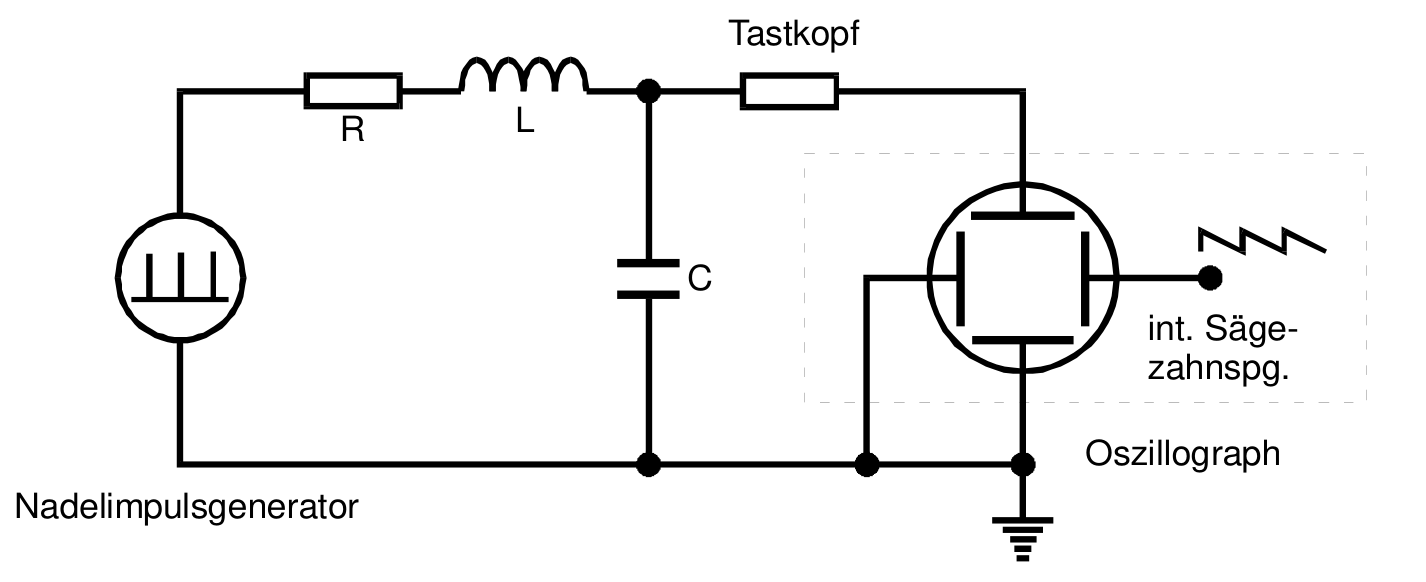
\includegraphics[width=0.7\textwidth]{Abbildungen/Schaltung_a.png}
    \caption{Schaltung für Aufgabe 1 \cite{man:v354}.}
    \label{fig:Schaltung_a}
\end{figure}
Das Oszilloskop wird mit einer Zeiteinheit (Timediv) von $\qty{20}{\micro\s}$
einer Spannungseinheit (Voltdiv) von $\qty{1}{\volt}$ pro Kästchen eingestellt.
Auf dem Oszilloskop wird eine kleiner werdende Schwingung erkannt.
Die Zeitpunkte und Auslenkungen dieser Peaks werden abgelesen und notiert.

\subsection{Widerstand des aperiodischen Grenzfalls}
Um den Widerstand zu ermitteln in dem der Aperiodische Grenzfall eintritt,
wird der Frequenzgenerator an einen einstellbaren Widerstand angeschlossen(vgl. Abb. \ref{fig:Schaltung_b}).
Die Einstellungen des Oszilloskops aus der vorherigen Aufgabe werden übernommen.
Der einstellbare Widerstand wird so lange erhöht, bis gerade keine Schwingungen mehr zu sehen sind.
Die Einstellung ist der Widerstand des aperiodischen Grenzfalls.
%%%%%%%%%%%%%%% blink
\begin{figure}
    \centering
    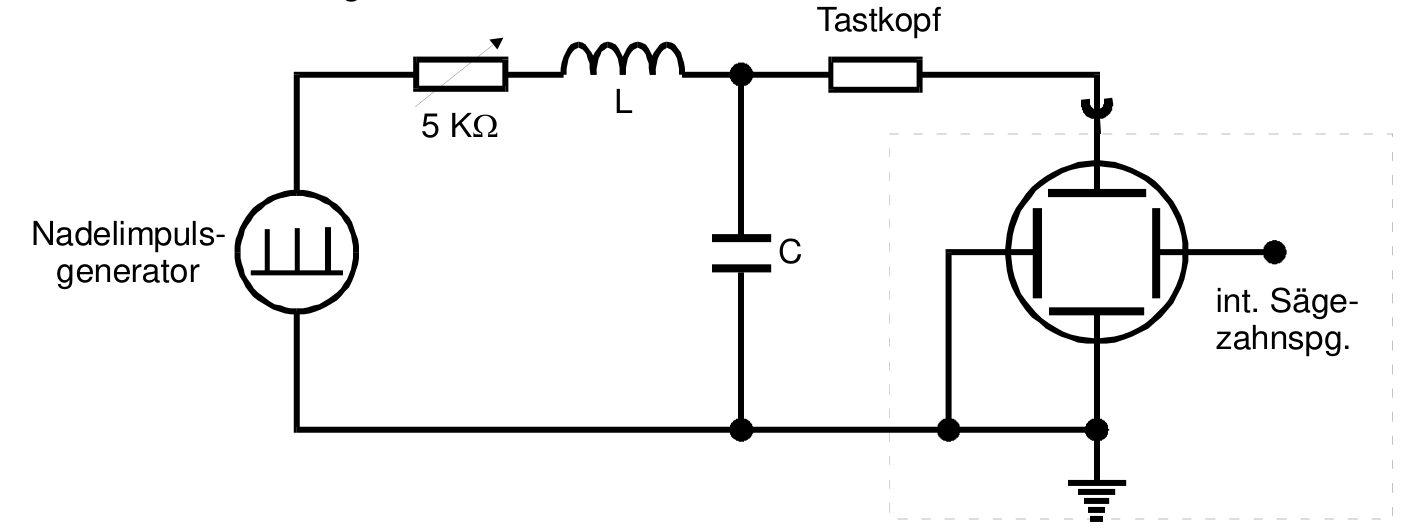
\includegraphics[width=0.7\textwidth]{Abbildungen/Schaltung_b.png}
    \caption{Schaltung für Aufgabe 2 \cite{man:v354}.}
    \label{fig:Schaltung_b}
\end{figure}


\subsection{Frequenzabhängigkeit von Amplitude und Phasenverschiebung bei der angetriebenen Schwingung}
Bei diesem Versuchsteil wird eine Sinusschwingung an den Schwingkreis mit dem
Widerstand $R_2$ angeschlossen um eine angetriebene gedämpfte Schwingung zu erzeugen (vgl. Abb. \ref{fig:Schaltung_c}).
%%%%%%%%%%%%%%% blink
\begin{figure}
    \centering
    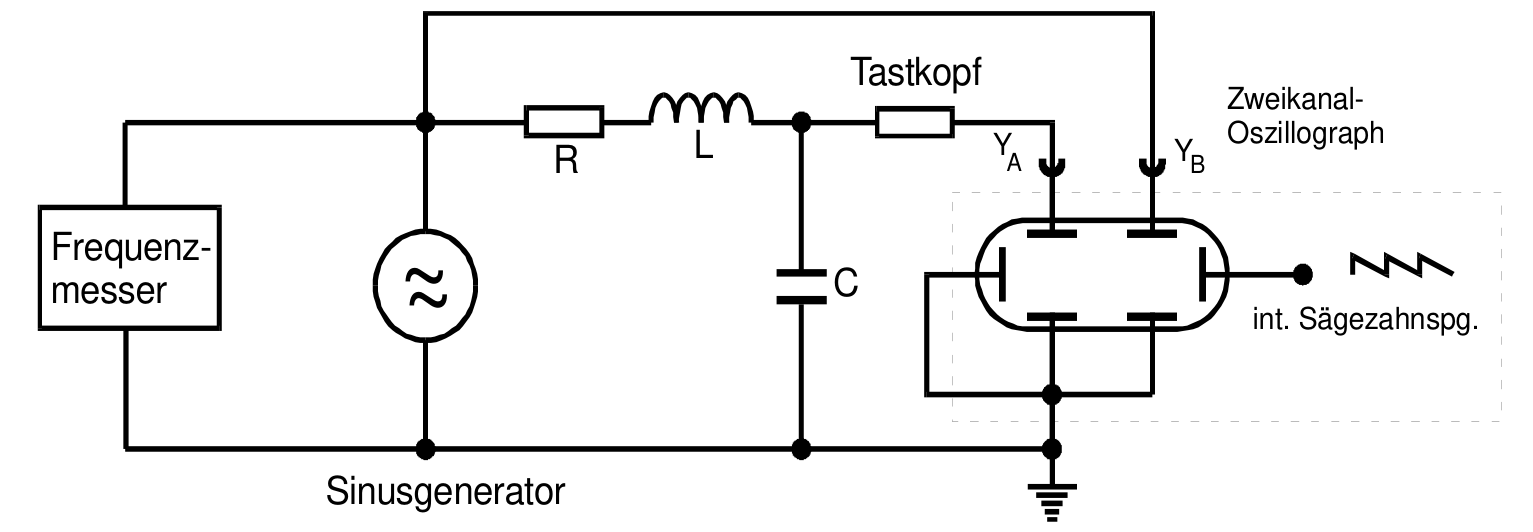
\includegraphics[width=0.7\textwidth]{Abbildungen/Schaltung_c.png}
    \caption{Schaltung für Aufgabe 3 \cite{man:v354}}
    \label{fig:Schaltung_c}
\end{figure}
Die Generatorspannung und die Spannung am Kondensator werden parallel auf dem Oszilloskop dargestellt.
Die Frequenzen werden nach und nach erhöht und die Amplitude der Spannung am Kondensator
sowie die Zeit des Phasenunterschieds wird aufgenommen.
Die an dem Oszilloskop gemessenen Werte sind durch eine falsche Einstellung am Fine-Tuning-Regler des Oszilloskops
in einer gleichbleibenden Art und Weise verzerrt.
Deshalb muss für den Phasenunterschied auch die Schwingungsdauer $T$ mit dem Oszilloskop gemessen werden, 
auch wenn diese aus der Frequenz hergeleitet werden könnte.